In the scope of supporting the configuration of a given product line some specific tools and techniques are used. This section gives an overview about the used techniques.

\subsection{Feature Models} \label{ch:fm}
\begin{figure}
	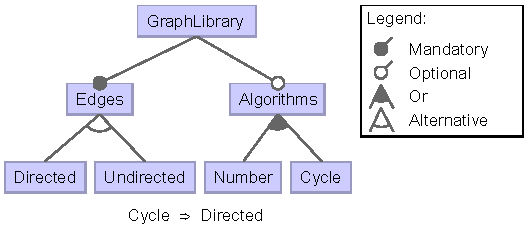
\includegraphics{img/img-fm.pdf}
	\caption{A simple example of a feature model}
	\label{img-fm}
\end{figure}

Feature models are a multi-purpose structure for product lines. One of their benefits is the visualization as a feature diagram, providing an overview of the containing features, and their hierarchy and dependencies. In addition, it classifies the features and their dependencies by ordinality, logical operator and whether it is abstract or concrete. Furthermore, it contains all information needed to provide a configuration of features and its validation. A configuration, or chosen set of features, is valid if there are no contradictions in the models dependencies or logical operators.

There are two main representations of feature models. The first approach is a propositional expression, which is a type of syntactic formula often used in propositional logic. However feature models are typically visualized in form of a feature diagram, which is structured as a tree \cite{fmgp}. In that manner feature models map the hierarchy of features. The possible relationships of features with a common parent feature are \textit{or}, \textit{alternative} and \textit{and}. All child features beneath a parent feature have the same relationship and therefore form a \textit{group}. In the case of an \textit{or}-group, at least one of the child features has to be selected if the parent feature is selected. Within an \textit{alternative}-group exactly one of the child feature has to be selected if the parent feature is selected. When features are grouped with an \textit{and}-relation, they are marked as either mandatory or optional. If the parent feature of an \textit{and}-group is selected, any number of optional marked features can be selected. Features marked as mandatory have to be selected. As features' relations may be of higher complexity than just parent-child relations additional constraints can be noted within a feature model. Constraints can contain any propositional expression.

In Figure~\ref{img-fm} we demonstrate an example of a simple feature model. The node \textit{GraphLibrary} is the root feature. It's childs are the node \textit{Edges}, that has to be selected due to the mandatory property, and \textit{Algorithms} that is marked optional. The implemented edge types are \textit{Directed} and \textit{Undirected} from which exactly one has to be chosen as they are mutually exclusive. From the algorithms at least one feature has to be chosen whenever \textit{Algorithms} is selected. The constraint at the bottom of Figure~\ref{img-fm} implies that if the feature \textit{Cycle} is selected, the edge type needs to be directed.


\subsection{Product Configuration}
The variability of a product line is represented by it's feature model, which itself is a set of features with specific interrelations. The configuration process of a product line describes the steps to derive a product from the product line. To archive this, a user has to select a subset of all the possible features within the product line to meet his requirements \cite{vrt}. However, not all subsets of features result in a valid product. The interrelations of the features restrict the possible combinations of features. Thus, not all arbitrary cobinations of features result in a \textit{valid} configuration. If only one of the requirements from the interrelations between the features is validated, no product can be created and the configuration as such is considered \textit{invalid}. For an automatic validity check, see the next section.

A non-final configuration, that is a configuration that still has some feature choices left to be made, is called a \textit{partial configuration}. A \textit{valid} partial configuration can be useful, as it narrows down the number of possible resulting variations and choices left to make. As the aim is to achieve a valid final configuration, there has to be a valid partial configuration after every choice made.


\subsection{Satisfiability} \label{ch:sat}
During creation of the feature model as well as during the configuration of a product, validity must always be taken care of. Validity in this context is described as the satisfiability of the corresponding propositional expression.

The formalism of propositional expressions (see Section~\ref{ch:fm}) allows feature models and configurations to be checked for validity. Each selected feature is appended with a logical \textit{AND} and each specifically unselected feature is also appended with a logical \textit{AND} but gets negated. The resulting expression is then evaluated by a SAT-solver to check for satisfiability \cite{sat-solve}. If the expression is satisfiable the selected features make up a valid configuration.

Even during configuration this process can be applied to check for invalid partial configurations after each decision. If a partial configuration reduces the valid choices in a group to a single one, this choice can be made automatically. This is called \textit{propagation}. The automatic selection or deselection of a features due to propagation of a made selection always results in a valid configuration \cite{fmi}.